\documentclass[11pt]{article}

\usepackage{float} % [H] option for tables
\usepackage{amssymb}
\usepackage{fullpage} % Use the full page
\usepackage{color}
\usepackage{tikz}
\usepackage[framed]{matlab-prettifier} % Matlab
\setlength\parindent{0pt} % No indentation


% Headers
\usepackage{fancyhdr}
\setlength{\headheight}{15.2pt}
\pagestyle{fancy}
\setlength\headsep{30pt}
\lhead{Youssef Beltagy}   					%  Your name on the left header.
\chead{\textsc{Vocoder Project}}			%  Title in the center.
\rhead{\today}							%  Date on the right header.

% Matlab blocks
\lstset{
  style              = Matlab-editor,
  basicstyle         = \mlttfamily,
  mlshowsectionrules = true,
  escapeinside={//}{//},
}

% Cover Page Settings
\title{
    \textsc{Vocoder Project Report}
}

\author{
    \Large{Youssef Beltagy} \\
    \large \textsc{AUT21 BEE 235}
}

\date{\today}

%--------------------------------------------
%%%%%%%%%%%%%%%%%%%%%%%%%%%%%%%%%%%%%%%%%%%%%%%%%%%%
% END OF THE PREAMBLE AND BEGINNING OF THE ACTUAL DOCUMENT
%%%%%%%%%%%%%%%%%%%%%%%%%%%%%%%%%%%%%%%%%%%%%%%%%%%%
%--------------------------------------------

\begin{document}


\maketitle % Make the cover page
\pagebreak


\section{Abstract}

I implemented a channel vocoder which can use a sine wave or
white noise as the carrier.
I experimented with the vocoder to identify the minimum number of 
bands necessary for a vocoded signal to be understandable.\\

I also implemented a sound chimaerizer which combines two sound signals
together to make a hybrid chimaera sound.

\section{Code Explanation}

This is a brief explanation of how the code is organized.\\

vocode.m and chimera.m are the vocoder and chimaerizer respectively.
vocode\_run and chimera\_run are helper functions to ease the use
of the vocoder and chimaerizer.\\

audioread\_mono.m loads an sound file as a mono channel audio signal.
bands\_cutoff.m generates the frequency ranges for the bands.
plots.m generates plots.
demo.m is a short demo of the code.\\

Please unzip the project and run demo.m.

\lstinputlisting{demo.m}

\section{Vocoder}

The vocoder splits the signal into frequency bands.
It then extracts the envelope of each band and multiplies the
envelope with a sine wave in the middle of the band.
The output signal is the summation of those bands.\\

\subsection{Sine Vocoder}

This is the output from the 4-band sine vocoder for ``The fire is very hot" (sentence 7).
It is similar to the input but it is more symmetric across the x-axis.

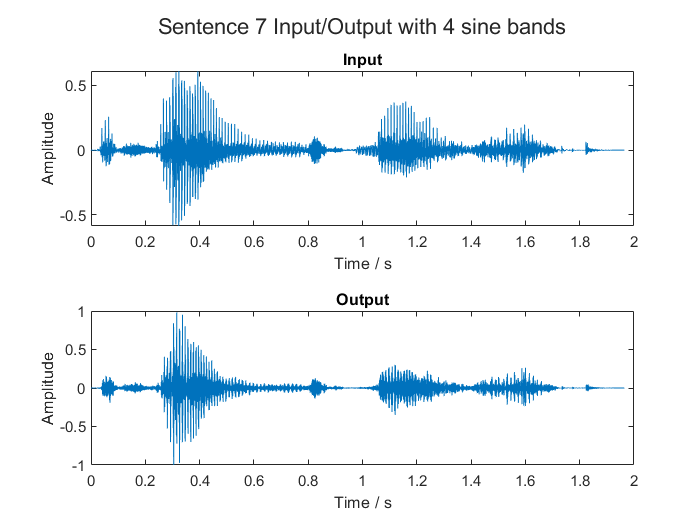
\includegraphics[height=0.3\textheight]{output/IO_4sine.png}

These are the envelopes used to generate the output.

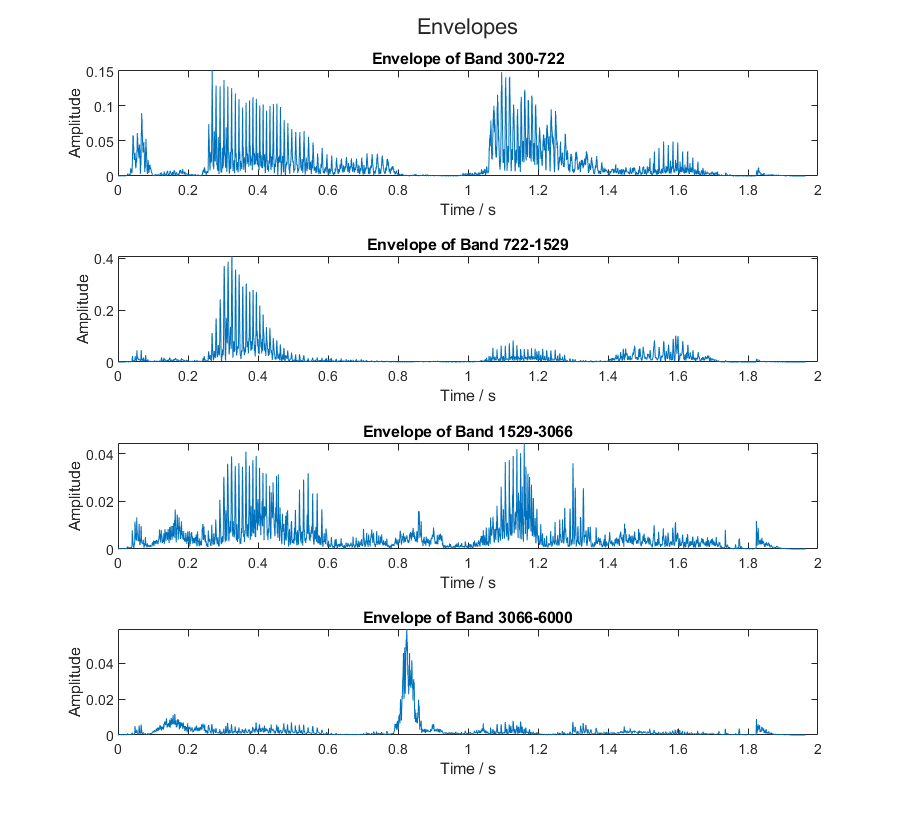
\includegraphics[height=0.45\textheight]{output/sent007_envelopes.png}

The below four images show the four bands generated when the vocoder
is used on ``The fire is very hot" with 4 frequency bands.
They show the everything starting from the original signal 
spectrum, to the band pass filter used, to the envelope of the band,
and to band itself.

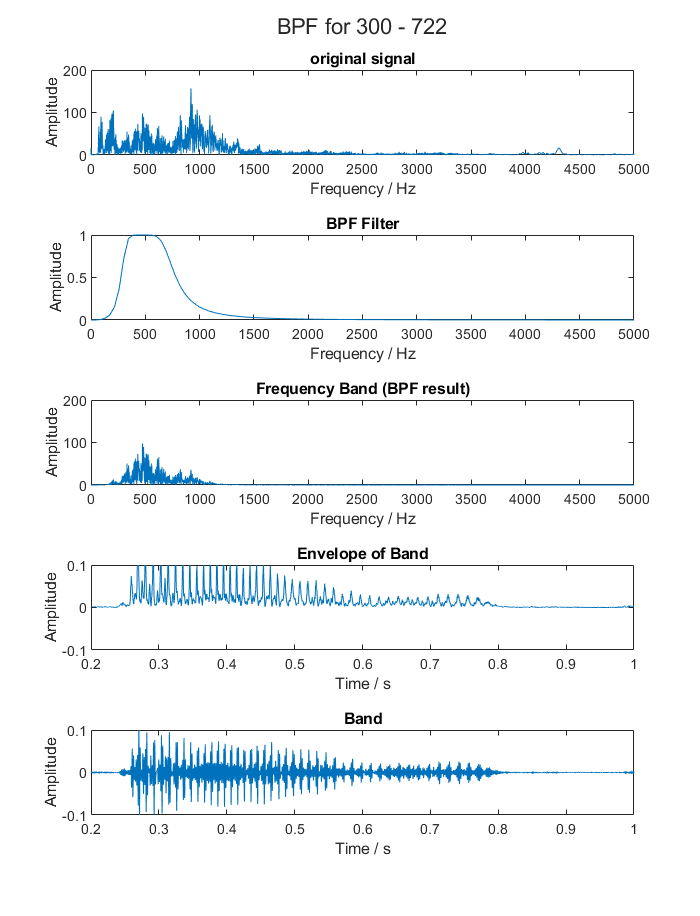
\includegraphics[height=\textheight]{output/band1.png}

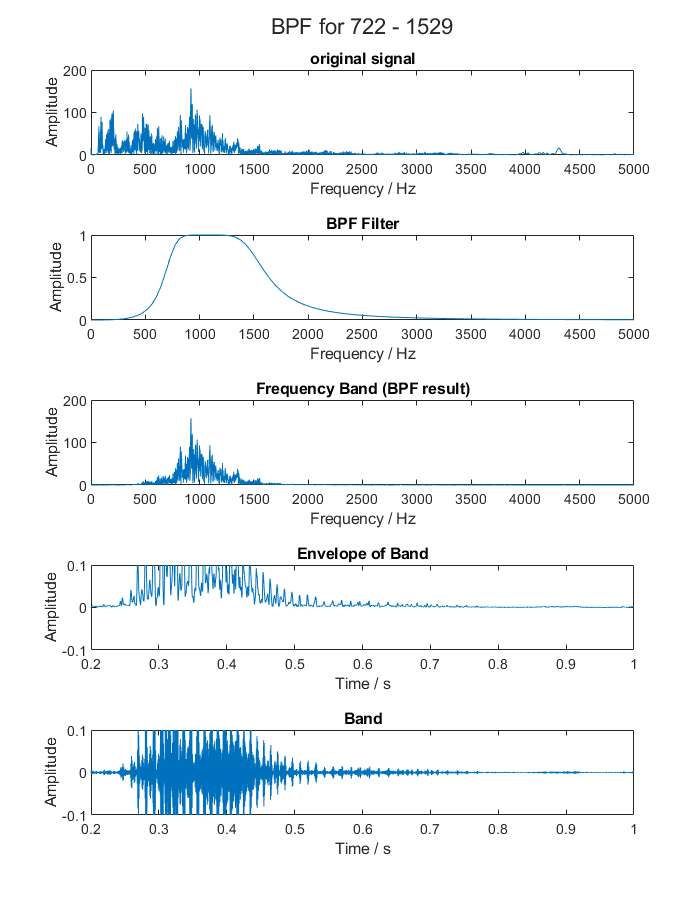
\includegraphics[height=\textheight]{output/band2.png}

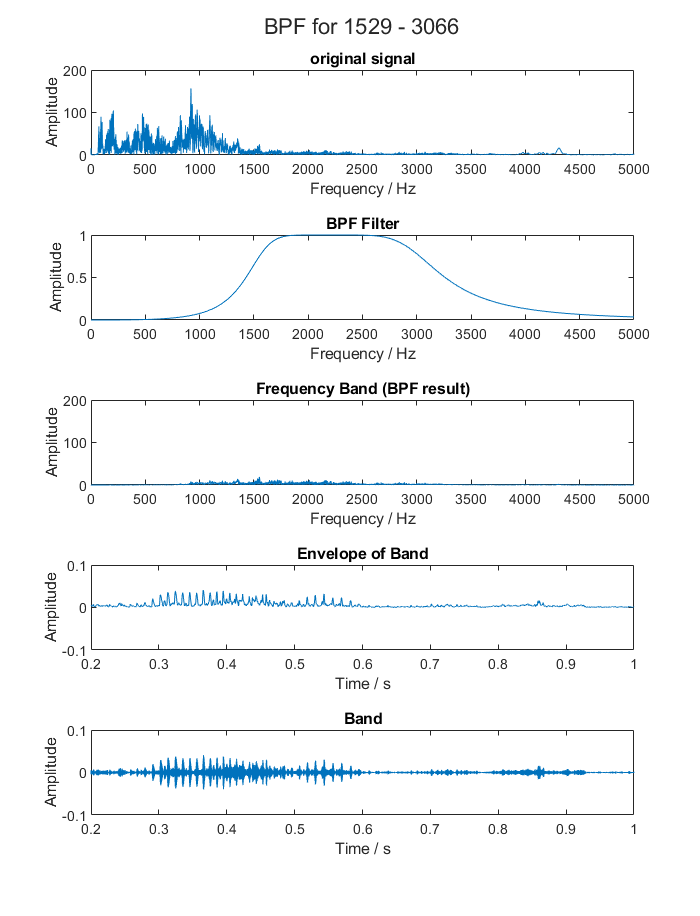
\includegraphics[height=\textheight]{output/band3.png}

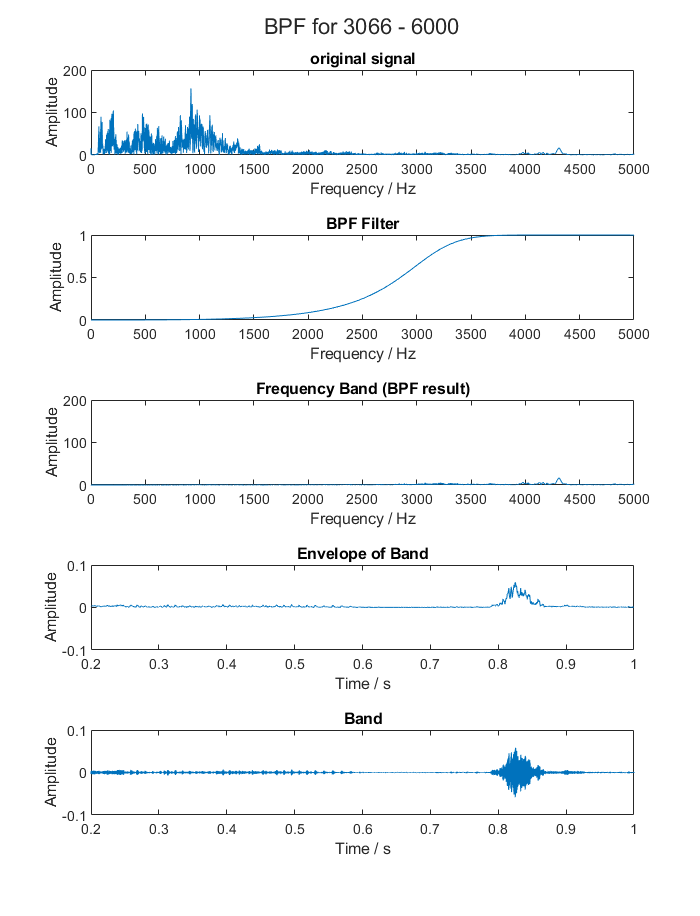
\includegraphics[height=\textheight]{output/band4.png}

To generate the envelopes, I use this low pass filter.

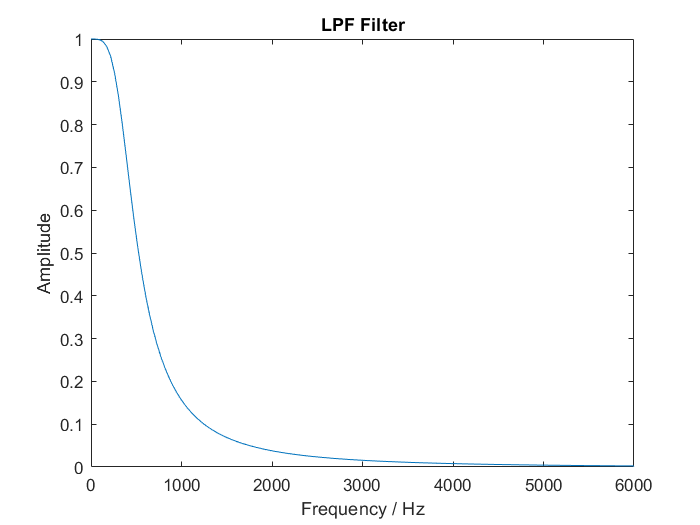
\includegraphics[width=\textwidth]{output/envelope_lpf.png}

\pagebreak
\subsection{White Noise Vocoder}

I implemented the white noise vocoder.
It is redundant to regenerate the previous plots for
the noise vocoder, so let's jump to the spectrum analysis.\\

This is the original signal spectrum.

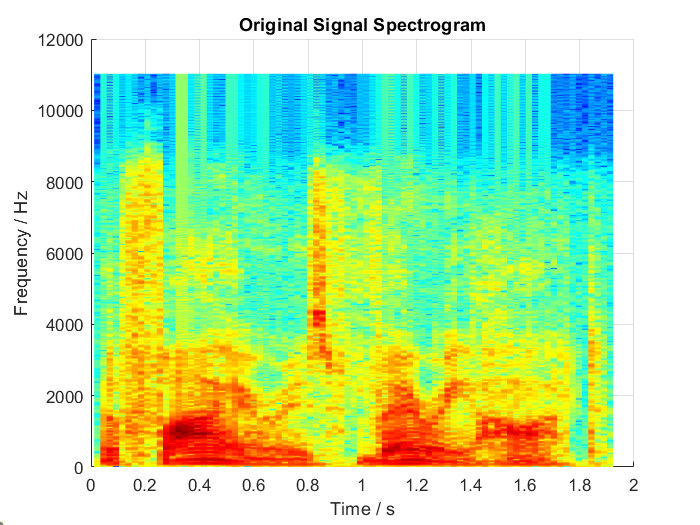
\includegraphics[height=0.4\textheight]{output/original_spectrogram.png}

The following two plots are the spectrograms of a 1-band and a 4-band sine vocoder, respectively.

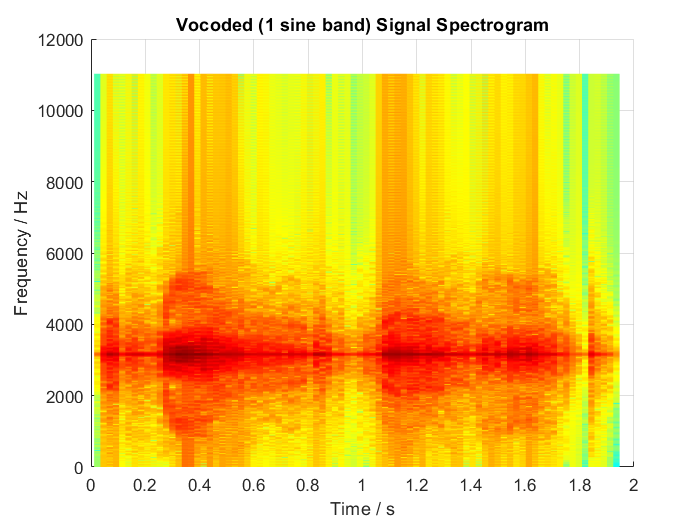
\includegraphics[height=0.4\textheight]{output/vocoded_1sine_spectrogram.png}

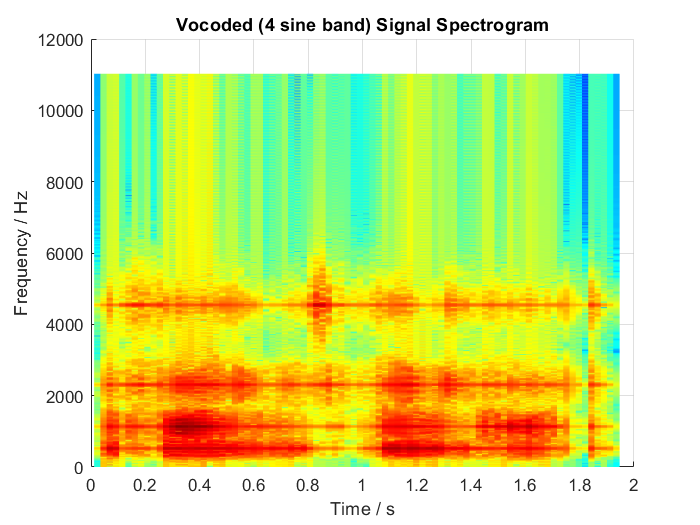
\includegraphics[height=0.4\textheight]{output/vocoded_4sine_spectrogram.png}

These last two plots are the spectrograms of a 1-band and a 4-band noise vocoder, respectively.

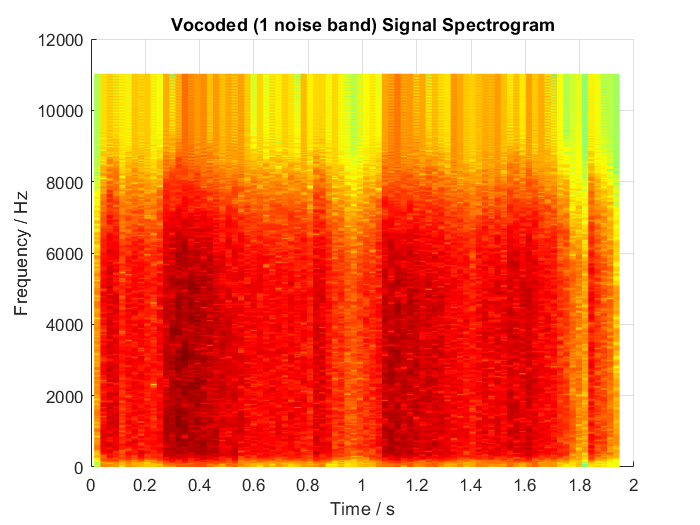
\includegraphics[height=0.4\textheight]{output/vocoded_1noise_spectrogram.png}

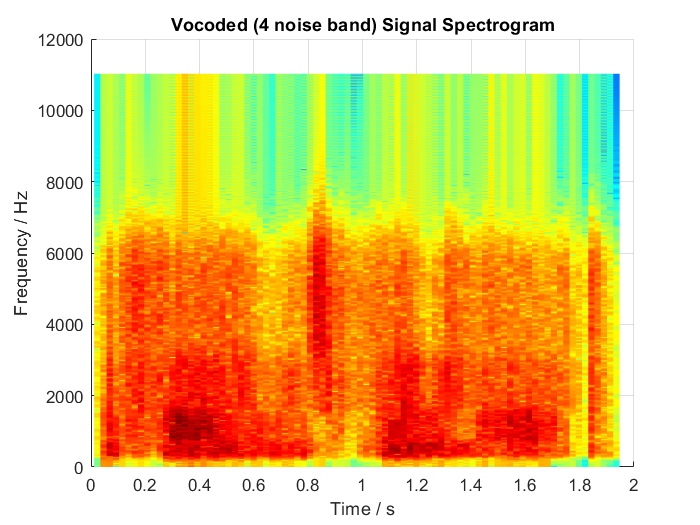
\includegraphics[height=0.4\textheight]{output/vocoded_4noise_spectrogram.png}

The sine vocoder has sharp horizontal lines for the sine of every band.
The noise vocoder's spectrum is much more uniform than the sine vocoder and looks more
similar to the original signal spectrum.

\pagebreak
\subsection{Sine Vocoder Experiment}

I asked two listeners to listen to sine vocoded sentences and tell
me the words they understood.
Since we were only provided with 15 sentences, I made more sentences with audacity.
They are open source and you can use them in future assignments.\\

The listeners started understanding the speech when the number of bands was 4.
But they felt very uncomfortable with 4 bands. They preferred 7-10 bands.\\

When the number of bands was in the hundreds (300 for example),
the listeners didn't understand the speech at all.

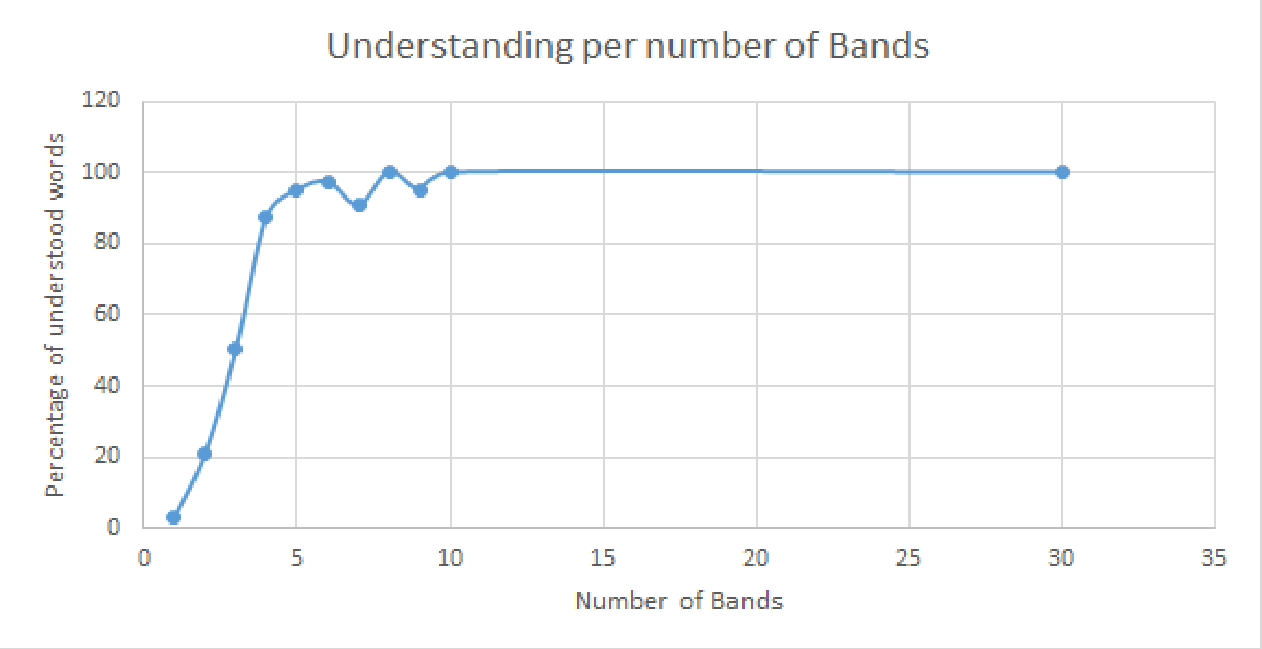
\includegraphics[width=\textwidth]{output/experiment.png}

\pagebreak
\section{Chimaerizer}
I implemented two versions of the chimaerizer:
One consistently uses one signal as the carrier and the other
as the envelope.
The other swaps the envelope and carrier between the two signals for 
every band.\\

Let's begin with the chimaerizer which doesn't swap.
If the two signals are the same, the output sounds just like the input.\\

If the two signals are different, but the number of bands is small (1-2),
the envelope is always more prominent than the carrier.
But as the number of bands increases, the carrier becomes more prominent.
When the number of bands is around 3-4, the two sounds are mixed together
and hard to understand.\\

When I played speech envelope with sound carrier,
it sounded as if background music was added to vocoded speech.\\

As for the chimaerizer which swaps,
for a small number of bands, the two signals mixed and were hard to discern.
When the number of bands is larger,
one signal seems to consistently win over the other.
I can then understand the winning signal.\\

Some signals keep switching between winning and losing.
In these cases, it sounded like two people are saying a sentence in turns (like the witches in Hercules)
and I confuse some words from one sentence with the other\\

 
When I played a sentence with music,
it sounded like someone synthesizing speech from music.\\

When I played two music signals together, it sounded like I was switching back and forth 
between two tracks.

\section{Conclusion}

I implemented a sine vocoder and a white noise vocoder.
Humans need at least 4 frequency bands to understand speech.
White noise vocoders are easier to understand than sine wave vocoders.\\

A chimaerizer mixes two sound signals together using one as an envelope
and the other as the carrier.
Chimaerizers make sounds which feel as if two people were talking at the same time.

\section{Code}

I attached the code in my submission, but I will include it here too for ease of reference.

\lstinputlisting{bands_cutoff.m}

\lstinputlisting{vocode.m}

\lstinputlisting{chimera.m}

\lstinputlisting{audioread_mono.m}

\lstinputlisting{vocode_run.m}

\lstinputlisting{chimera_run.m}

\lstinputlisting{plots.m}

\end{document}
